\documentclass[11pt,letterpaper]{report}
\usepackage[pdftex]{graphicx}
\usepackage[version=3]{mhchem}
\usepackage{tabularx}
\usepackage{latexsym}
\usepackage{multirow}

\newcommand{\HRule}{\rule{\linewidth}{0.5mm}}
\setlength{\topmargin}{-.7in}
\setlength{\leftmargin}{-.7in}
\setlength{\textheight}{9in}
\setlength{\oddsidemargin}{0in}
\setlength{\textwidth}{6.25in}



%_{()}

%\multicolumn{4}{|l|}{\ce{}} \\

\begin{document}

\begin{titlepage}
\begin{center}

\textsc{\Large Lab 4}\\[1.5cm]
\textsc{\Large Grossmont College - Chemistry 141}\\[0.5cm]

\HRule \\[0.4cm]
{ \LARGE \bfseries Redox Reactions: The Activity Series}\\[0.5cm]

\HRule \\[1.5cm]

\begin{minipage}{0.4\textwidth}
\begin{flushleft} \large
\emph{Author:}\\
Cameron \textsc{Carroll}
\end{flushleft}
\end{minipage}
\begin{minipage}{0.4\textwidth}
\begin{flushright} \large
\emph{Instructor \& Class:}\\
Judy \textsc{George} - 141 (8844)
\end{flushright}
\end{minipage}

\vfill

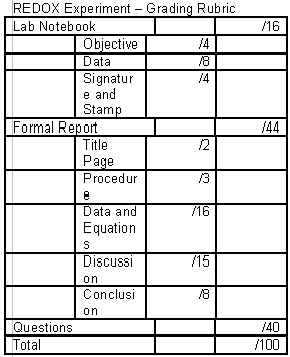
\includegraphics{./redox_rxn_rubric.png}\\[1cm]

{\large \today}

\end{center}
\end{titlepage}
\pagebreak

\section*{Objective}
The Redox Reaction experiments are intended to provide the basis for exploration of the relative reactivity of a set of elements. This data will be used to construct an activity series. 

\section*{Data}
\begin{tabularx}{\textwidth}{ | X| X| X| X| }
\hline
\textsc{Reaction ($\uparrow$)} &\textsc{Element Reduced} & \textsc{Oxidizing Agent} & \textsc{More Active} \\
\hline
\multicolumn{4}{|l|}{\ce{Cu_{(s)} + ZnSO4_{(aq)} -> \textsc{No Reaction}}} \\
\hline
 & nil & Cu & Zn \\
\hline
\multicolumn{4}{|l|}{\ce{Cu_{(s)} + FeSO4_{(aq)} -> \textsc{No Reaction}}} \\
\hline
 & nil & Cu & Fe \\
\hline
\multicolumn{4}{|l|}{\ce{Zn_{(s)} + CuSO4_{(aq)} -> ZnSO4_{(aq)} + Cu_{(s)}}} \\
\hline
 & Cu & Cu & Zn \\
\hline
\multicolumn{4}{|l|}{\ce{Zn_{(s)} + FeSO4_{(aq)} -> ZnSO4_{(aq)} + Fe_{(s)} }} \\
\hline
& Fe & Fe & Zn \\
\hline
\multicolumn{4}{|l|}{\ce{Fe_{(s)} + CuSO4_{(aq)} -> FeSO4_{(aq)} + Cu_{(s)}}} \\
\hline
 & Cu & Cu & Fe \\
\hline
\multicolumn{4}{|l|}{\ce{Fe_{(s)} + ZnSO4_{(aq)} -> \textsc{No Reaction}}} \\
\hline
 & nil & Fe & Zn \\
\hline
\multicolumn{4}{|l|}{\ce{Cu_{(s)} + H2SO4_{(aq)} -> \textsc{No Reaction}}} \\
\hline
 & nil & Cu & H+ \\
\hline
\multicolumn{4}{|l|}{\ce{Zn_{(s)} + H2SO4_{(aq)} -> ZnSO4_{(aq)} + H2_{(g)}}} \\
\hline
 & H & H & Zn \\
\hline
\multicolumn{4}{|l|}{\ce{Fe_{(s)} + H2SO4_{(aq)} -> FeSO4_{(aq)} + H2_{(g)}}} \\
\hline
 & H & H & Fe \\
\hline
\multicolumn{4}{|l|}{\ce{I2_{(aq)} + Br-_{(aq)} -> \textsc{No Reaction}}} \\
\hline
 & nil & I & Br \\
\hline
\multicolumn{4}{|l|}{\ce{Br2_{(aq)} + I-_{(aq)} -> Br-_{(aq)} + I2_{(aq)}}} \\
\hline
 & Br & Br & Br \\
\hline
\multicolumn{4}{|l|}{\ce{FeCl3_{(aq)} + KBr_{(aq)} -> \textsc{No Reaction}}} \\
\hline
 & nil & Fe & Br \\
\hline
\multicolumn{4}{|l|}{\ce{FeCl3_{(aq)} + KI_{(aq)} -> FeI2_{(aq)} + KCl_{(aq)}}} \\
\hline
 & Fe & Fe & Fe \\
\hline
\end{tabularx}

\section*{Discussion}
Some of the results in the data collected are rather confusing; Where a reaction theoretically should have occured, I found only minor bubbles on the metal. Therefore, the inequalities supporting by that observation are weaker than the others in this experiment (\ce{Zn + FeSO4}, \ce{Zn + H2SO4} \& \ce{Fe + H2SO4}) Some of the other reactions' observations include the finish wearing off of the piece of metal, which may or may not be a sign of a chemical reaction. There is a possibility of error due to forgetting to sand down the surfaces of metal before reacting them.

\section*{Conclusion}
The final hierarchy for reaction series is: \ce{Zn -> Br -> Fe -> H+ -> Cu -> I}. (From most reactive to least reactive.) This seems reasonable, although it contains implied solutions; Not every chemical was tested against oneanother... I, for example, is only tested against two, and its reactivity against the remainder must be inferred. 


\end{document}